%------------------- Bearings and Spacers -------------------%
\subsection{Bearings and Spacers} \label{subsec:bearings}

%------------------------------ Inputs and Outputs ------------------------------%
\subsubsection{Inputs and Outputs}
This section shows the analysis of the sleeve bearings (bushings) and gives specifications for the spacers on the shafts. The main input for the bearings is the shaft diameter and the radial forces at the bearings (calculated in shaft analysis). The output is the required length of the bearing. Spacers are not highly critical, but are included in this section to specify basic geometries and materials.

%------------------------------ CONSTANTS ------------------------------%
\subsubsection{Constants and Parameters}
For these analysis' the shaft diameters (found in the shaft analysis) are considered as constants. 
For the safety factor, the same value as the shafts (2.5) will be aimed for.


%------------------------------ Assumptions ------------------------------%
\subsubsection{Assumptions and Simplifications}
Friction in the sleeve bearings is neglected as its exact value was difficult to calculate and the worst case value calculated was relatively small. See the attempted calculations in Appendix \ref{app:bearing_friction}.

The sleeve bearings are chosen to have a constant thickness, as this does not affect their performance as per the calculations. A thickness of 2 mm was chosen based on existing sleeve bearings \cite{quality_bearings_and_components_flanged_nodate} and the fact that we will likely have very short bushings. The bearings will also have a flange to help position them in the housing and on the shafts as well as take the minor axial loads coming from the legs. As the axial loads are not very large, the size of the flange was not based on analysis and is simply based on the size of the shaft step and thickness of the spacer that will be in contact with the flange. 

As the spacers are not taking excessive axial loads, their thickness is chosen as 5 mm. This value is expected to be sufficient to maintain the axial position of parts, while also keeping the bushing flange at a reasonable size. 

%------------------------------ Materials ------------------------------%
\subsubsection{Material Selection}
The sleeve bearings were chosen as sintered bronze bearings. The reason for this selection is that this is a common and well-known material, is corrosion resistant and is self-lubricating. The useful properties of bronze for the analysis are $P_{material}=55 MPa$ and $PV_{material}=1.8 MPa \;m/s$. A lighter material, such as plastic, might have been chosen, however these are more limited in temperature ranges and their weight difference is not considerable for a small bushing. The sleeve bearings are press fit into their respective housing, and the shaft is inserted inside with a clearance fit.

The spacers are selected to be made of polycarbonate, as it is lightweight, thermally stable, can take impact forces and is moisture resistant \cite{omnexus_polycarbonate_nodate}. 

%------------------------------ Stress Analysis ------------------------------%
\subsubsection{Stress Analysis and Free-Body Diagrams}

The diagram in \ref{fig:bearing_dimensions} shows the important dimensions of the sleeve bearing for the calculations.

\begin{figure}
    \centering
    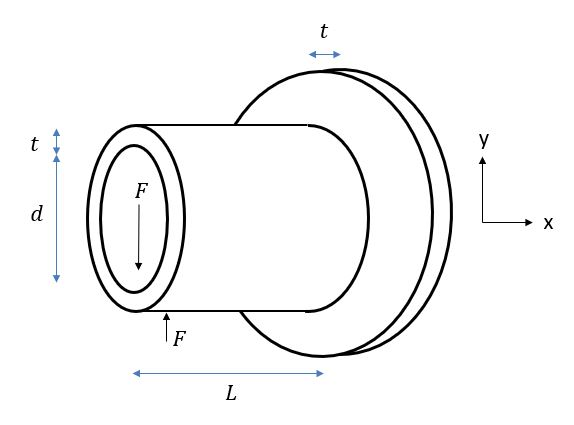
\includegraphics[width=0.6\textwidth]{4_Analysis/img/Bearing/bearing.JPG}
    \caption{Sleeve Bearing - Dimensional diagram}
    \label{fig:bearing_dimensions}
\end{figure}

where $L$ is the sleeve bearing length, $d$ is the inner diameter (shaft diameter for simplification) and $t$ is the thickness of the bearing wall (constant).

The original analysis was done for roller bearings, where it was found that these were not adequate for the static forces encountered in this application (see Appendix \ref{app:ball_bearing}).

Instead, the sleeve bearings (bushings) were chosen, as they can take more radial forces. The method used to determine the required length of the sleeve bearing is the pressure-velocity ($PV$) factor \cite{daemar_inc_bushing_2013}. This value is a material property and is described by Equation \ref{eq:bearing_PV}. As this application uses very low velocities, the pressure ($P$) is also observed. This is done using Equation \ref{eq:bearing_pressure}. Analysing the velocity is unnecessary for this case, as the application is close to static.

\begin{gather}
    P=\frac{F}{dL} \label{eq:bearing_pressure}
    \\
    V=\frac{\pi{}dn}{60\times10^3} \label{eq:bearing_velocity}
    \\
    PV=\frac{\pi{}Fn}{60\times10^3L} \label{eq:bearing_PV}
\end{gather}

where $F$ is the radial force acting on the bearing in N and $n$ is the rotational speed of the shaft in rpm. The rotational speed is assumed as the maximum value reached during a cycle. This gives a somewhat conservative estimate of the pressure-velocity factor.

The following is an example where the exterior knee shaft sleeve bearing length is found. This shaft has the highest forces on its bearings due to belt tension and forces from the leg. Equations \ref{eq:bearing_pressure} and \ref{eq:bearing_PV} are rearranged to get the minimal required length of the bearing. To do so, the bearing material properties are used: bronze has operating limits of $P_{material}=55 MPa$ and $PV_{material}=1.8 MPa \;m/s$. Other values are $d = 13.0 mm$ (from shaft analysis Section \ref{sec:shaft_example}), $n = 1.60 rpm$ (maximum rotational speed from modelling) and $F = 1124.1 N$ (the combination of the forces acting on the bearing in x and y from the shaft analysis, using Equation \ref{eq:Ftotal}).

\begin{gather}
    L_{required}=\frac{F}{dP_{material}}=\frac{1124.1 N}{13.0 mm \times 55 MPa}=1.57 mm
    \\
    L_{required}=\frac{\pi{}Fn}{60\times10^3PV_{material}}=\frac{\pi\times1124.1 N\times 1.60 rpm}{60\times 1000 \times 1.8 MPa\;m/s}=0.05 mm
\end{gather}

Thus we choose the largest value of 1.57 mm and apply the safety factor to get $L$. This value is quite close to the value assumed for the shaft calculations, which was 4.0 mm, thus we can round up to this value. 

\begin{equation}
    L=SF\times L_{required}=2.5\times 1.57 mm = 3.93 mm \approx 4.0 mm
\end{equation}


%------------------------------ Critical Review ------------------------------%
\subsubsection{Critical Review}
The bearing lengths make sense as the chosen material is quite strong for this application, meaning that only small lengths are required. The thickness of the flange (2 mm) also contributes to the length of the bearing but removes some length from the part of the sleeve bearing radially in contact with the housing. It will likely be required to choose longer bearings due to this. 

%------------------------------ Parameterization ------------------------------%
\subsubsection{Parameterization}
The parameterization goal will be to find the required length of the bearing for the applied bearing forces, which depend highly on the weight of the robot. A value for the length of the bearing will need to be estimated for the shaft analysis in order to find bearing forces, and then the assumed length will be modified following the bearing analysis. It will be an iterative process. 
However, as seen in the example with the worst case scenario, the length of the bearings is already quite small. Another option would be to simply set a length that works for all situations, and keep it constant without parameterization. Otherwise, a minimum sleeve bearing length will be set to ensure stability and manufacturability of the assembly (for example, the hip shaft bearings take very low load, thus we would limit the bearing length to a minimum of 3 mm).